\section{Auswertung}
\label{sec:Auswertung}

\subsection{Berechnung der theoretischen Fourier-Koeffizienten}
\subsubsection{Rechteckspannung}
Die zeitabhängige Funktion f(t) der Rechteckspannung wird definiert als:
\[
f(t)=
	\begin{cases}
     -U_.0 & \text{für } -\frac{T}{2}+nT \textless t \textless nT\\
     0  & \text{für } x=n\frac{T}{2} \\
     U_.0  & \text{für } nT \textless t \textless \frac{T}{2}+nT 
   	\end{cases}
\hspace{2em},n\in N
\]
Dabei entspricht $T$ der Periodendauer und $U_.0$ der Amplitude der Spannung. Da die Funktion ungerade definiert wurde, sind alle Koeffizienten $\mathrm{a}_n=0$ und die $\mathrm{b}_n$ ergeben sich nach Formel \eqref{eq:Koeffizienten} zu:
\begin{equation}
\mathrm{b}_n =
	\begin{cases} 
	\frac{4U_.0}{\pi n} & \text{bei ungeradem }n\\
	0 & \text{bei geradem }n
	\end{cases}
\label{eq:KoeffRechteck}
\end{equation}

\subsubsection{Sägezahnspannung}
Die zeitabhängige Funktion f(t) der Sägezahnspannung wird definiert als:
\[
f(t)=
	\begin{cases}
     \frac{2U-.0}{T}t-U_.0 & \text{für } -\frac{T}{2}+nT \textless t \textless nT\\
     0  & \text{für } x=nT
   	\end{cases}
\hspace{2em},n\in N
\]
Dabei entspricht $T$ der Periodendauer und $U_.0$ der Amplitude der Spannung. Da die Funktion ungerade definiert wurde, sind alle Koeffizienten $\mathrm{a}_n=0$ und die $\mathrm{b}_n$ ergeben sich nach Formel \eqref{eq:Koeffizienten} zu:
\begin{equation}
\mathrm{b}_n = \frac{-2U_.0}{\pi n} 
\label{eq:KoeffSägezahn}
\end{equation}

\subsubsection{Dreieckspannung}
Die zeitabhängige Funktion f(t) der Dreieckspannung wird definiert als:
\[
f(t)=
	\begin{cases}
     \frac{4U-.0}{T}t-U_.0 & \text{für } nT \le t \textless \frac{T}{2}+nT\\
     \frac{-4U-.0}{T}t+3U_.0 & \text{für } \frac{T}{2}+nT \le t \textless nT
   	\end{cases}
\hspace{2em},n\in N
\]
Dabei entspricht $T$ der Periodendauer und $U_.0$ der Amplitude der Spannung. Da die Funktion gerade definiert wurde, sind alle Koeffizienten $\mathrm{b}_n=0$ und die $\mathrm{a}_n$ ergeben sich nach Formel \eqref{eq:Koeffizienten} zu:
\begin{equation}
\mathrm{a}_n =
	\begin{cases} 
	\frac{-8U_.0}{\pi^2 n^2} & \text{bei ungeradem }n\\
	0 & \text{bei geradem }n
	\end{cases}
\label{eq:KoeffDreieck}
\end{equation}

\subsection{Fourier-Analyse}
\subsubsection{Rechteckspannung}
Der Funktionsgenerator wird auf eine Frequenz $f=\SI{50e3}{\hertz}$ und eine Spannung von $U_.{Rechteck} = \SI{1e3}{\volt}$ eingestellt.
Aus den gemessenen Daten wird das Amplitudenverhältnis $\frac{U_.n}{U_.1}$ der $n$ten Oberwelle zur Grundschwingung bestimmt, was in Tabelle \ref{tab:tab1} zu sehen ist.

\begin{table}
	\centering
	\caption{Messdaten der Oberwellen einer Rechteckspannung.}
	\sisetup{table-format=1.2}
	\begin{tabular}{S[table-format=2.0] S[table-format=3.1]S[table-format=3.1]S[table-format=1.2]}
		\toprule
		{$n$}&{$\nu/10^3\si[per-mode=reciprocal]{\hertz}$}&{$U_.n/\si[per-mode=reciprocal]{\volt}$}&{$\frac{U_.n}{U_.1}$} \\
		\midrule
		1 & 43,8 & 424,0 & 1,00 \\
		3 & 146,8 & 144,0 & 0,34 \\
		5 & 234,3 & 80,0 & 0,19 \\
		7 & 337,5 & 62,8 & 0,15 \\
		9 & 431,2 & 41,6 & 0,10 \\
		11 & 528,1 & 40,0 & 0,09 \\
		13 & 631,2 & 30,6 & 0,07 \\
		15 & 718,7 & 28,4 & 0,07 \\
		17 & 818,7 & 24,4 & 0,06 \\
		\bottomrule
	\end{tabular}
	\label{tab:tab1}
\end{table}

\noindent In Abbildung \ref{fig:R} wird das Amplitudenverhältnis gegen die Anzahl der Oberwellen halblogarithmisch aufgetragen. Die Regression 
\begin{equation}
\frac{U_.n}{U_.1}(n) = a \cdot n^{-b}\label{eq:Reg}
\end{equation}
liefert für den Koeffizienten:
\[
b_.{Rechteck,mess}= 1,01 \pm 0,01\text{.}
\]
Nach \eqref{eq:KoeffRechteck} fällt die Kurve einer Rechteckspannung mit $\frac{1}{n}$ ab, also gilt:
\[
b_.{Rechteck,theo}= 1\text{.}
\]
Die Abweichung beträgt somit
\[
\Delta b = 1\% \text{.}
\]

\begin{figure}
\centering
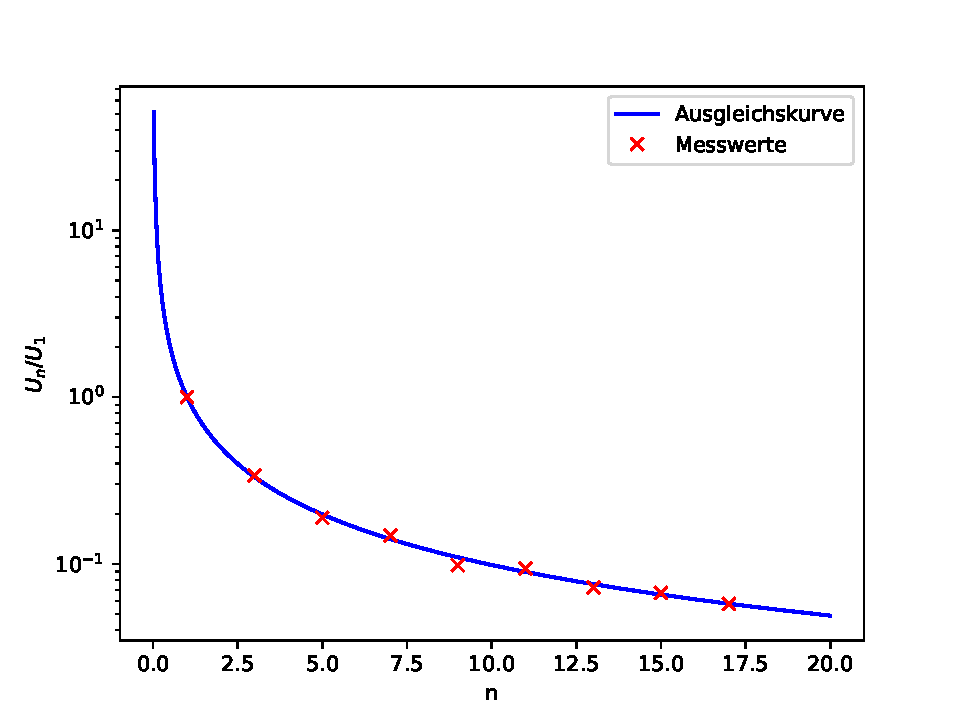
\includegraphics[width=\linewidth-75pt,height=\textheight-75pt,keepaspectratio]{content/images/rechteck.pdf}
\caption{Rechteck-Amplitudenverhältnis in Abhängigkeit von der Zahl der Oberwelle.}\label{fig:R}
\end{figure}

\subsubsection{Sägezahnspannung}
Der Funktionsgenerator wird auf eine Frequenz $f=\SI{100e3}{\hertz}$ und eine Spannung von $U_.{Saegezahn} = \SI{1e3}{\volt}$.\newline
Aus den gemessenen Daten wird das Amplitudenverhältnis $\frac{U_.n}{U_.1}$ der $n$ten Oberwelle zur Grundschwingung bestimmt, was in Tabelle \ref{tab:tab2} zu sehen ist. In Abbildung \ref{fig:S} wird das Amplitudenverhältnis gegen die Anzahl der Oberwellen halblogarithmisch aufgetragen. Die Regression nach Gleichung \eqref{eq:Reg} liefert:
\[
b_.{Sägezahn,mess} = 1,00 \pm 0,02\text{.}
\]
Dies entspricht dem Theoriewert 
\[
b_.{Sägezahn,theo} = 1,
\]
da nach \eqref{eq:KoeffSägezahn} die Kurve mit $\frac{1}{n}$ abnimmt.

\begin{table}
	\centering
	\caption{Messdaten der Oberwellen einer Sägezahnspannung.}
	\sisetup{table-format=1.2}
	\begin{tabular}{S[table-format=1.0] S[table-format=3.1]S[table-format=3.1]S[table-format=1.2]}
		\toprule
		{$n$}&{$\nu/10^3\si[per-mode=reciprocal]{\hertz}$}&{$U_.n/\si[per-mode=reciprocal]{\volt}$}&{$\frac{U_.n}{U_.1}$} \\
		\midrule
		1 & 87,5 & 208,0 & 1,00 \\
		2 & 187,5 & 96,0 & 0,46 \\
		3 & 287,5 & 72,0 & 0,35 \\
		4 & 387,5 & 54,4 & 0,26 \\
		5 & 487,5 & 40,4 & 0,19 \\
		6 & 587,5 & 34,0 & 0,16 \\
		7 & 681,2 & 32,0 & 0,15 \\
		8 & 781,2 & 26,6 & 0,13 \\
		9 & 875,0 & 21,4 & 0,10 \\
		\bottomrule
	\end{tabular}
	\label{tab:tab2}
\end{table}

\begin{figure}
\centering
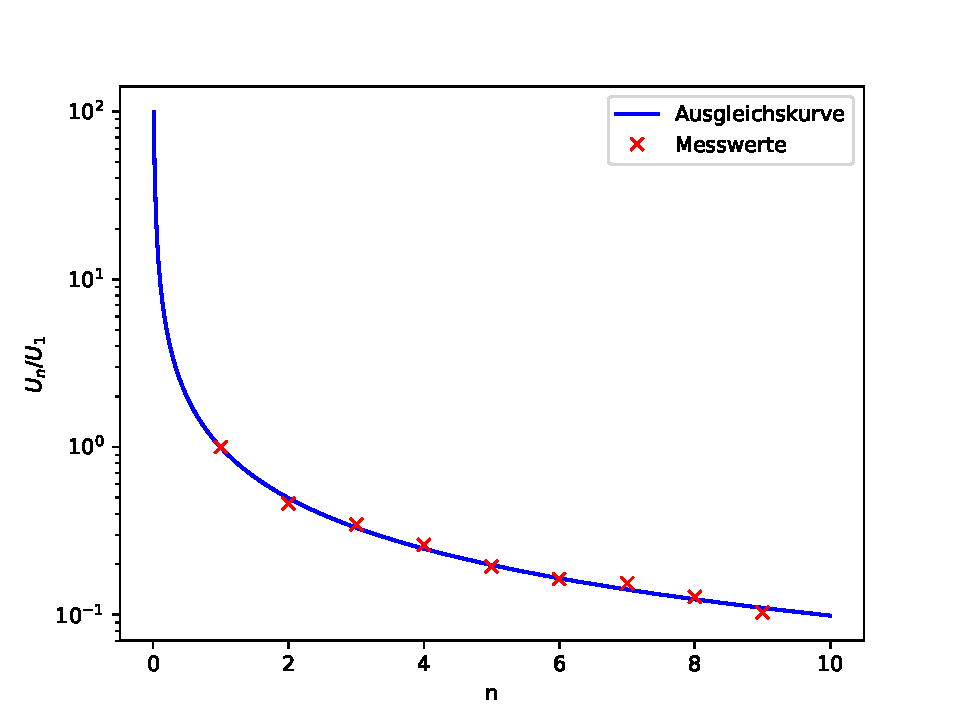
\includegraphics[width=\linewidth-75pt,height=\textheight-75pt,keepaspectratio]{content/images/saegezahn.pdf}
\caption{Sägezahn-Amplitudenverhältnis in Abhängigkeit von der Zahl der Oberwelle.}\label{fig:S}
\end{figure}

\subsubsection{Dreieckspannung}
Der Funktionsgenerator wird auf eine Frequenz $f=\SI{100e3}{\hertz}$ und eine Spannung von $U_.{Dreieck} = \SI{1e3}{\volt}$.\newline
Aus den gemessenen Daten wird das Amplitudenverhältnis $\frac{U_.n}{U_.1}$ der $n$ten Oberwelle zur Grundschwingung bestimmt, was in Tabelle \ref{tab:tab3} zu sehen ist.

\begin{table}
	\centering
	\caption{Messdaten der Oberwellen einer Dreieckspannung.}
	\sisetup{table-format=1.2}
	\begin{tabular}{S[table-format=2.0] S[table-format=4.0]S[table-format=3.1]S[table-format=3.1]}
		\toprule
		{$n$}&{$\nu/10^3\si[per-mode=reciprocal]{\hertz}$}&{$U_.n/\si[per-mode=reciprocal]{\volt}$}&{$\frac{U_.n}{U_.1}/10^{-2}$} \\
		\midrule
		1 & 85 & 270,0 & 100,0 \\
		3 & 245 & 29,8 & 11,0 \\
		5 & 405 & 11,0 & 4,1 \\
		7 & 565 & 5,0 & 1,9 \\
		9 & 725 & 3,4 & 1,3 \\
		11 & 885 & 2,0 & 0,7 \\
		13 & 1045 & 1,8 & 0,7 \\
		15 & 1205 & 1,3 & 0,5 \\
		\bottomrule
	\end{tabular}
	\label{tab:tab3}
\end{table}

\noindent In Abbildung \ref{fig:D} wird das Amplitudenverhältnis gegen die Anzahl der Oberwellen halblogarithmisch aufgetragen. Die Regression nach Gleichung \eqref{eq:Reg} liefert:
\[
b_.{Sägezahn,mess} = 2,01 \pm 0,01\text{.}
\]
Da die Dreieckspannung nach \eqref{eq:KoeffDreieck} theoretisch mit $\frac{1}{n^2}$ abfällt, gibt es eine Abweichung zum Theoriewert
\[
b_.{Sägezahn,theo} = 2
\]
von
\[
\Delta b = 0,5\% \text{.}
\]

\begin{figure}
\centering
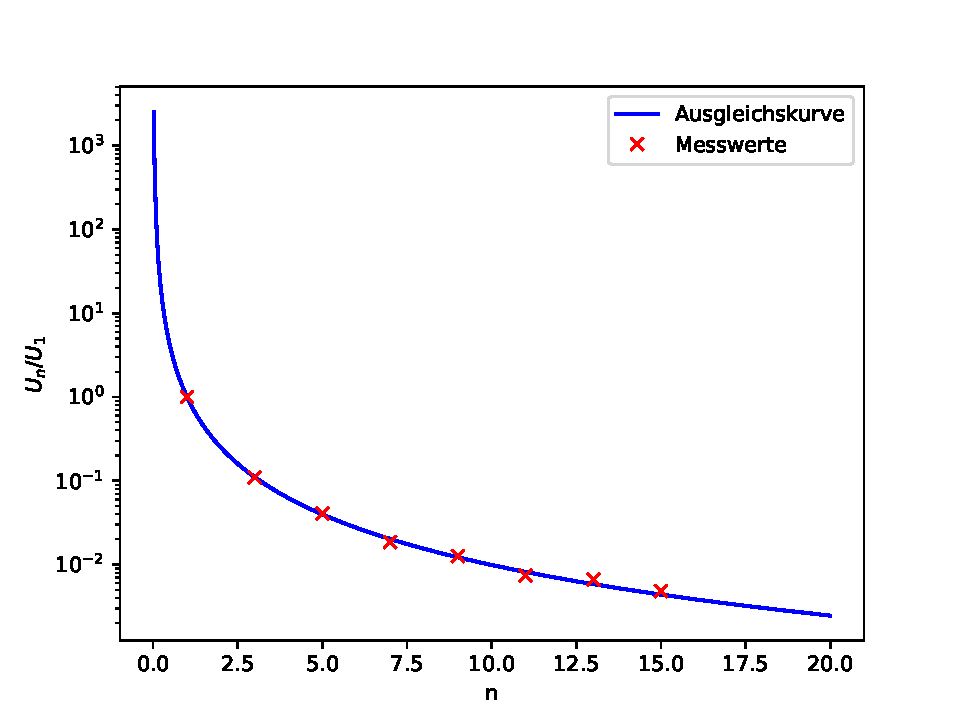
\includegraphics[width=\linewidth-75pt,height=\textheight-75pt,keepaspectratio]{content/images/dreieck.pdf}
\caption{Dreieck-Amplitudenverhältnis in Abhängigkeit von der Zahl der Oberwelle.}\label{fig:D}
\end{figure}

\subsection{Fourier-Synthese}
Bei allen Synthesen wurden die einzelnen Oberwellen über die Lissajous-Figuren so justiert, dass das bestmögliche Resultat erreicht wurde.
\subsubsection{Rechteckspannung}
Eine Rechteckspannung von $\SI{100}{\volt}$ wird aus den in Tabelle \ref{tab:tab4} aufgezählten Oberwellen synthetisiert. Das Ergebnis ist in Abbildung \ref{fig:R2} zu sehen.

\begin{table}
	\centering
	\caption{Einstellungen zur Synthese einer Rechteckspannung.}
	\sisetup{table-format=1.2}
	\begin{tabular}{S[table-format=1.0] S[table-format=3.1]}
		\toprule
		{$n$}&{$U/\si[per-mode=reciprocal]{\volt}$}\\
		\midrule
		1 & 127,0 \\
		3 & 42,4 \\
		5 & 25,5 \\
		7 & 18,2 \\
		9 & 14,1 \\
		\bottomrule
	\end{tabular}
	\label{tab:tab4}
\end{table}

\begin{figure}
\centering
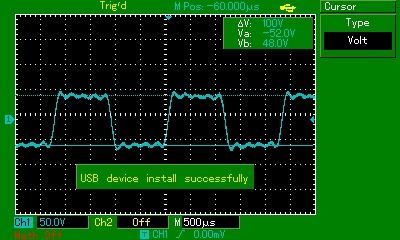
\includegraphics[width=\linewidth-75pt,height=\textheight-75pt,keepaspectratio]{content/images/rechteck.jpg}
\caption{Synthetisierte Rechteckspannung.}
\label{fig:R2}
\end{figure}

\subsubsection{Sägezahnspannung}
Eine Sägezahnspannung von $\SI{100}{\volt}$ wird aus den in Tabelle \ref{tab:tab5} aufgezählten Oberwellen synthetisiert. Das Ergebnis ist in Abbildung \ref{fig:S2} zu sehen.

\begin{table}
	\centering
	\caption{Einstellungen zur Synthese einer Sägezahnspannung.}
	\sisetup{table-format=1.2}
	\begin{tabular}{S[table-format=1.0] S[table-format=2.1]}
		\toprule
		{$n$}&{$U/\si[per-mode=reciprocal]{\volt}$}\\						\midrule
		1 & 63,7 \\
		2 & 31,8 \\
		3 & 21,2 \\
		4 & 15,9 \\
		5 & 12,7 \\
		6 & 10,6 \\
		7 & 9,1 \\
		8 & 8,0 \\
		9 & 7,1 \\
		\bottomrule
	\end{tabular}
	\label{tab:tab5}
\end{table}

\begin{figure}
\centering
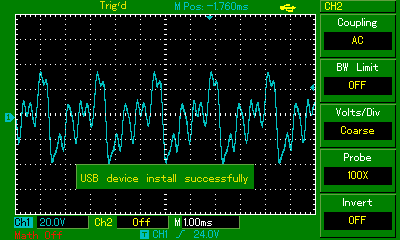
\includegraphics[width=\linewidth-75pt,height=\textheight-75pt,keepaspectratio]{content/images/saegezahn.jpg}
\caption{Synthetisierte Sägezahnspannung.}
\label{fig:S2}
\end{figure}

\subsubsection{Dreieckspannung}
Eine Dreieckspannung von $\SI{157}{\volt}$ wird aus den in Tabelle \ref{tab:tab6} aufgezählten Oberwellen synthetisiert. Das Ergebnis ist in Abbildung \ref{fig:D2} zu sehen.
\begin{table}
	\centering
	\caption{Einstellungen zur Synthese einer Dreieckspannung.}
	\sisetup{table-format=1.2}
	\begin{tabular}{S[table-format=1.0] S[table-format=3.1]}
		\toprule
		{$n$}&{$U/\si[per-mode=reciprocal]{\volt}$}\\
		\midrule
		1 & 127,3 \\
		3 & 14,1 \\
		5 & 5,1 \\
		7 & 2,6 \\
		\bottomrule
	\end{tabular}
	\label{tab:tab6}
\end{table}

\begin{figure}
\centering
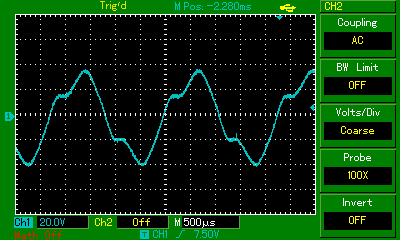
\includegraphics[width=\linewidth-75pt,height=\textheight-75pt,keepaspectratio]{content/images/dreieck.jpg}
\caption{Synthetisierte Dreieckspannung.}\label{fig:D2}
\end{figure}